%% IJCAI-format METHOD paper, first draft (v0.1). Experiments are still running: every number marked
%% \pilot comes from a single training seed; cells marked \tbd are filled when the runs finish.
%% Upload the official IJCAI author-kit files (ijcai27.sty or ijcai26.sty, named.bst) next to this file.
\IfFileExists{ijcai27.sty}{\def\ijcaistyle{ijcai27}}{\IfFileExists{ijcai26.sty}{\def\ijcaistyle{ijcai26}}{}}
\ifdefined\ijcaistyle
  \documentclass{article}
\else
  \documentclass[twocolumn,10pt]{article}
\fi
\pdfpagewidth=8.5in
\pdfpageheight=11in
\ifdefined\ijcaistyle
  \usepackage{\ijcaistyle}
\else
  \usepackage[letterpaper,margin=0.75in,columnsep=0.25in]{geometry}
  \usepackage[round]{natbib}
\fi
\usepackage{times}
\usepackage{soul}
\usepackage{url}
\usepackage[utf8]{inputenc}
\usepackage[small]{caption}
\usepackage{graphicx}
\usepackage{amsmath}
\usepackage{amssymb}
\usepackage{booktabs}
\usepackage{xcolor}
\usepackage{algorithm}
\usepackage{algpseudocode}
\urlstyle{same}

\newcommand{\todo}[1]{\textcolor{red}{[TODO: #1]}}
\newcommand{\tbd}{\textcolor{red}{TBD}}
\newcommand{\pilot}{\textsuperscript{\textcolor{gray}{$\dagger$}}}
\newcommand{\sg}{\operatorname{sg}}
\newcommand{\JS}{\operatorname{JS}}
\newcommand{\ours}{PGCT}

\title{Learning Whom to Share With:\\ Policy-Gated Critic Transfer for Multi-Agent Reinforcement Learning with Latent Teams}
\author{Anonymous submission}

\begin{document}
\maketitle

\begin{abstract}
When several groups of learning agents share an environment, each with its own objective, sharing knowledge
between agents can accelerate learning---but only between the right agents, and in practice team membership
is often unknown. We propose Policy-Gated Critic Transfer (\ours{}), a decentralised method in which each agent
decides from local interactions whose value estimates to learn from. Neighbouring agents compare their action
distributions on a fixed, pre-agreed bank of probe observations; a smoothed Jensen--Shannon gate selects
compatible partners, and the agent distils their critics on the probe inputs while its actor and its own
experience remain private. No team labels, raw observations or parameters are exchanged. On a two-team
multi-robot warehouse task trained from scratch, preliminary results \todo{seed 1 only; update with seeds 2--$n$}
show that \ours{} reaches one delivery per episode 13\% earlier than independent PPO, achieves 12\% higher
average throughput over training and 18\% higher final throughput, and closes most of the gap to an oracle that
shares only with ground-truth teammates (89\% of its average throughput), whereas indiscriminate sharing with
every neighbour delays learning by two million steps. Selective sharing mainly helps agents that fall behind:
under \ours{} three of four agents learn the task, compared with two under independent learning. We analyse
which partners the gate selects and evaluate \ours{} on a variant in which the teams' goals diverge
\todo{E1-F results}.
\end{abstract}

\section{Introduction}
Many multi-agent systems consist of several groups that pursue different objectives in a shared space:
warehouse robots of different clients, vehicles of different fleets, or teams of players. Agents in such
systems learn simultaneously and observe each other only locally. Sharing learned knowledge---parameters,
experience or value estimates---is one of the most effective ways to improve sample efficiency in multi-agent
reinforcement learning (MARL) \cite{christianos2020seac,christianos2021seps}. Yet sharing presupposes
compatibility: knowledge from an agent that pursues a different objective, or that has learned something
different, can mislead the learner. When group membership is latent, every agent faces the question
\emph{whom should I learn from?}

Existing answers either assume the groups are known, cluster agents with a centralised procedure
\cite{christianos2021seps,hu2025heterogeneity}, or share with every agent in a communication graph
\cite{zhang2018networked}. We study the decentralised case: each agent must decide from its own local
interactions, without team labels, a central coordinator, or access to other agents' observations.

We propose \textbf{Policy-Gated Critic Transfer (\ours{})}. Its key idea is that two agents can compare their
policies without exchanging experience: if both evaluate a fixed, pre-agreed bank of probe observations, the
divergence between their action distributions measures how differently they would act in the same situations.
A smoothed threshold on this divergence gates \emph{critic distillation}: the receiver regresses its value
predictions on the probe inputs towards those of selected neighbours. Sharing only critics keeps actors and
experience private and lets each agent remain an independent learner; sharing only with selected neighbours
avoids importing incompatible value estimates.

Our contributions are:
\begin{itemize}
  \item \ours{}, a decentralised, label-free partner-selection and critic-transfer method that exchanges only
    model outputs on a shared probe bank (Section~\ref{sec:method}).
  \item An evaluation protocol for selective sharing that compares against no sharing (IPPO), indiscriminate
    sharing (All-peer) and privileged team sharing (Oracle-team) from identical initial weights and logs the
    realised transfer at every update (Section~\ref{sec:setup}).
  \item Preliminary evidence on a two-team warehouse task that selective sharing outperforms both no sharing and
    indiscriminate sharing and approaches oracle sharing, chiefly by helping lagging agents learn
    (Section~\ref{sec:results}). \todo{confirm with seeds 2--$n$ and E1-F}
  \item An analysis of which partners the gate selects: in a team-symmetric task it links agents with similar roles
    across teams, consistent with independently measured critic compatibility (Section~\ref{sec:analysis}).
\end{itemize}

\section{Related Work}
\textbf{Parameter and experience sharing.} Parameter sharing is the default in cooperative MARL but forces
homogeneous behaviour. SePS clusters agents by an encoding of their transitions learned before training and
shares parameters within clusters \cite{christianos2021seps}; heterogeneity-aware methods decide dynamically
which agents share \cite{hu2025heterogeneity}. SEAC shares experience between agents with importance weighting
\cite{christianos2020seac}. These methods share actors or data and typically rely on centralised clustering;
\ours{} shares only critic predictions and selects partners locally and online.

\textbf{Decentralised critics.} Networked actor-critic methods drive critic parameters to consensus over a
communication graph \cite{zhang2018networked}. \ours{} instead decides per neighbour whether to transfer at all,
transfers through distillation on probe inputs \cite{rusu2016policy}, and allows individual rewards.

\textbf{Roles and independent learning.} Role-based methods discover roles from action effects
\cite{wang2021rode}; we find that a policy-similarity gate behaves partly like a role detector.
Independent PPO is a strong baseline in cooperative MARL \cite{schulman2017ppo,dewitt2020ippo}; centralised-critic
methods such as MAPPO \cite{yu2022mappo} use more information than our setting allows and are reported as
reference baselines \todo{MAPPO, SePS-style, HetDPS-style results}. We follow the evaluation recommendations of
\cite{agarwal2021precipice}.

\section{Problem Setting}
We consider a partially observable stochastic game with agents $i\in\{1,\dots,N\}$, local observation histories
$h_i^t$, actions $a_i^t$ and individual rewards $r_i^t$. Each agent belongs to a latent team $z_i\in\{1,\dots,K\}$
that determines its objective. An agent knows its own objective through team-relative observations but does not
observe $z_j$ of other agents. Agents within communication range form a time-varying neighbourhood
$\mathcal{N}_i(t)$ and can exchange low-dimensional model outputs; they do not exchange observations, experience,
parameters or team labels. Each agent learns its own policy $\pi_i$ and critic $V_i$. The goal is sample
efficiency: maximise every agent's return within a fixed budget of environment steps.

\section{Policy-Gated Critic Transfer}
\label{sec:method}
\textbf{Probe bank.} All agents hold the same bank $\mathcal{Q}=\{q_m\}_{m=1}^{M}$ of probe observations,
generated by a deterministic rule from the environment layout before training (in our experiments $M=48$
single-step observations covering pickup, delivery and return situations). Probes are evaluated with a zero
initial recurrent state, so a probe query is a single forward pass.

\textbf{Policy distance.} Every $P$ updates, neighbours $i$ and $j$ exchange their action distributions on the
bank and compute
\begin{equation}
  D_{ij} = \frac{1}{M}\sum_{m=1}^{M} \JS\big(\pi_i(\cdot\mid q_m),\, \pi_j(\cdot\mid q_m)\big).
\end{equation}
Because agents meet irregularly, the distance is smoothed only when they are neighbours,
$\bar D_{ij}\leftarrow(1-\beta)\bar D_{ij}+\beta D_{ij}$.

\textbf{Gate and allocation.} After a warm-up of $U_0$ updates and at least $n_{\min}$ measurements, agent $i$
selects the neighbours $\mathcal{G}_i(t)=\{j\in\mathcal{N}_i(t): \bar D_{ij}<\tau\}$ and weights them uniformly,
$\alpha_{ij}=1/|\mathcal{G}_i(t)|$ for $j\in\mathcal{G}_i(t)$. The gate is evaluated by each receiver, so transfer
can be asymmetric.

\textbf{Critic distillation.} The receiver adds a distillation term to its PPO objective,
\begin{equation}
  \mathcal{L}_i = \mathcal{L}^{\mathrm{PPO}}_i + \lambda_{\mathrm{peer}} \sum_{j\in\mathcal{G}_i(t)} \alpha_{ij}\,
  \frac{1}{M}\sum_{m=1}^{M}\big(V_i(q_m) - \sg[V_j(q_m)]\big)^2 ,
  \label{eq:loss}
\end{equation}
where $\sg$ is the stop-gradient and donor values are fixed at the start of the update. Only the receiver's
critic is affected; its actor is trained on its own experience.

\textbf{Communication.} Per probe round, a pair exchanges $M\,|\mathcal{A}|$ action probabilities and, when
transfer is active, $M$ value predictions (here $48\times5$ and $48$ numbers). No observations, gradients or
parameters are exchanged.

\begin{algorithm}[t]
\caption{\ours{} for agent $i$}
\label{alg:pgct}
\begin{algorithmic}[1]
\State Initialise $\pi_i, V_i$; $\bar D_{ij}\gets$ undefined for all $j$
\For{update $u=1,2,\dots$}
  \State Collect a rollout with $\pi_i$; compute PPO targets from own rewards
  \If{$u \bmod P = 0$}
    \For{$j\in\mathcal{N}_i(t)$}
      \State Exchange $\pi(\cdot\mid q_m)$ on $\mathcal{Q}$; update $\bar D_{ij}$
    \EndFor
  \EndIf
  \State $\mathcal{G}_i\gets\{j\in\mathcal{N}_i(t): \bar D_{ij}<\tau\}$ if $u>U_0$, else $\emptyset$
  \State Receive $V_j(q_m)$ from $j\in\mathcal{G}_i$
  \State Update $\pi_i, V_i$ on $\mathcal{L}_i$ (Eq.~\ref{eq:loss})
\EndFor
\end{algorithmic}
\end{algorithm}

\section{Experimental Setup}
\label{sec:setup}
\textbf{Environment.} We use a two-team variant of the multi-robot warehouse \cite{papoudakis2021benchmarking}
on an $11\times10$ map (\emph{E1}) with four agents (agents 1, 3 in team red; 2, 4 in team blue). Each team
always has two outstanding shelf requests and its own delivery goal; the goals are adjacent at the bottom centre,
and half of each team's shelves lie in the other team's half of the map. Observations are egocentric $11\times11$
semantic grids with team-relative channels (``requested shelf'', ``relevant goal''). Rewards are individual: an agent
is rewarded for its own deliveries and returns plus small shaping terms. In \emph{E1-F} the team goals are moved to
opposite bottom corners, so that the teams' objectives lead to different behaviour.

\textbf{Methods.} All methods use independent recurrent PPO actors and critics and differ only in the donor set:
\textbf{IPPO} (none), \textbf{All-peer} (every neighbour), \textbf{Oracle-team} (neighbours with the same
ground-truth team; privileged reference), and \textbf{\ours{}}. \ours{} uses $P=5$, $\beta=0.35$, $\tau=0.12$,
$U_0=100$, $n_{\min}=8$ and $\lambda_{\mathrm{peer}}=0.01$; all other hyper-parameters are shared (Appendix~A).
\ours{}-v2 additionally uses separate probe banks for the gate (agents carrying a shelf with no goal in view) and
for distillation (balanced over task phases) \todo{E1-F results}.

\textbf{Protocol.} All agents are trained from random initialisation; for a given seed all methods start from
bit-identical weights. Policies are evaluated every 51{,}200 environment steps on 20 episodes of 500 steps with a
deterministic masked policy and fixed reset seeds. We report the delivery onset (first step at which the 3-point
moving average reaches one delivery per episode), the mean deliveries per episode over training (normalised area
under the learning curve), the final deliveries (mean of the last five evaluations), and the number of agents that
learned the task. The realised donor allocation is logged at every update.
\textbf{Status of results.} The E1 comparison currently has one training seed and was stopped at 6.5M steps; all
statistics use the common horizon of 6.4M steps and are marked \pilot. \todo{seeds 2--$n$ at 10M; E1-F at 10M}

\section{Results}
\label{sec:results}

\begin{table}[t]
\centering
\small
\resizebox{\columnwidth}{!}{%
\begin{tabular}{lcccccc}
\toprule
Method & Labels & Onset$\downarrow$ & Mean$\uparrow$ & Final$\uparrow$ & Learned & Mean ($n$ seeds) \\
\midrule
IPPO & -- & 2.05M & 10.4 & 23.2 $\pm$ 1.1 & 2/4 & \tbd \\
All-peer & -- & 3.99M & 3.7 & 19.4 $\pm$ 1.6 & 4/4 & \tbd \\
\textbf{\ours{} (ours)} & -- & 1.79M & 11.7 & 27.3 $\pm$ 1.4 & 3/4 & \tbd \\
\midrule
Oracle-team & team & 1.64M & 13.2 & 32.2 $\pm$ 1.7 & 3/4 & \tbd \\
\bottomrule
\end{tabular}}
\caption{E1, trained from scratch, one seed\pilot, common horizon 6.4M steps. Onset: steps to one delivery per
episode. Mean: average deliveries per episode over training. Final: last five evaluations (mean $\pm$ s.d.\ over
evaluations, not seeds). Learned: agents with at least one delivery per episode at the end. Oracle-team uses
ground-truth team labels. Last column: to be filled with mean and 95\% interval over seeds.}
\label{tab:main}
\end{table}

\begin{figure}[t]
\centering
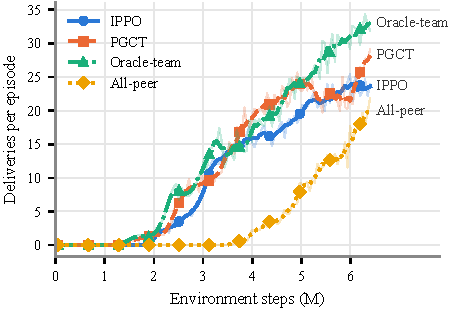
\includegraphics[width=\columnwidth]{figures/fig1_learning_curves.pdf}
\caption{Evaluation deliveries per episode on E1 (one seed\pilot). Thin lines: raw evaluations every 51{,}200
steps; thick lines: centred 5-point moving average.}
\label{fig:curves}
\end{figure}

\textbf{Main comparison.} Table~\ref{tab:main} and Figure~\ref{fig:curves} summarise the E1 comparison.\pilot{}
\ours{} improves on independent learning on every measure: it reaches one delivery per episode 0.26M steps
(13\%) earlier, its average throughput over training is 12\% higher (11.7 vs.\ 10.4 deliveries per episode) and its
final throughput 18\% higher (27.3 vs.\ 23.2). It was also the first method to reach 20 deliveries per episode
(4.15M steps vs.\ 4.66M for Oracle-team and 5.07M for IPPO). Without access to team labels, \ours{} attains 89\% of
the average throughput of Oracle-team. Indiscriminate sharing is clearly harmful early: All-peer reaches one
delivery per episode only after 3.99M steps, two million steps after the other methods, although it was improving
fastest when the run ended. In this run, selectivity rather than sharing per se made the difference.

\begin{figure*}[t]
\centering
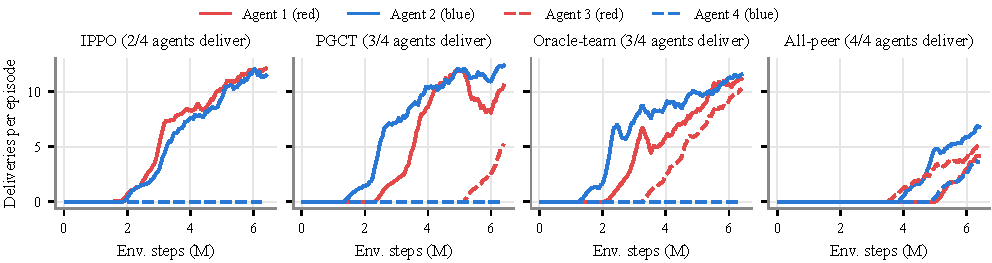
\includegraphics[width=\textwidth]{figures/fig2_per_agent_deliveries.pdf}
\caption{Deliveries per episode of each agent (5-point moving average; one seed\pilot). Red: team red (agents 1, 3);
blue: team blue (agents 2, 4); solid: agents 1--2; dashed: agents 3--4.}
\label{fig:agents}
\end{figure*}

\textbf{Selective sharing helps lagging agents.} The per-agent curves (Figure~\ref{fig:agents}) show where the gain
comes from. Under IPPO only one agent per team learned to deliver; the other two kept moving but never picked up a
requested shelf. With individual rewards and two requests per team, the first teammate to learn serves most
requests and the second receives too little reward to learn from. Critic distillation gives the lagging agent a
value signal without its own rewards: under \ours{} and Oracle-team a third agent learned (agent 3, from 5.4M and
3.6M steps respectively), and under All-peer all four did, albeit late. Each agent that learned contributed about
10--12 deliveries per episode, so the number of learning agents explains most of the throughput differences.
\todo{intervention: block distillation to the lagging agent; count learners over seeds}

\begin{table}[t]
\centering
\small
\resizebox{\columnwidth}{!}{%
\begin{tabular}{lcccc}
\toprule
 & \multicolumn{2}{c}{E1 ($11\times10$)} & \multicolumn{2}{c}{E2 ($16\times16$)} \\
\cmidrule(lr){2-3}\cmidrule(lr){4-5}
Method & AUC & Last 10 & AUC & Last 10 \\
\midrule
IPPO & 44.57 & 44.52 & 34.24 & 37.61 \\
\ours{} & 45.86 & 46.17 & 34.17 & 37.47 \\
\bottomrule
\end{tabular}}
\caption{Continuation for 4M steps from a shared curriculum checkpoint (one seed\pilot). AUC: normalised area under
the evaluation-delivery curve; Last 10: mean of the last ten evaluations. This earlier experiment used learning rate
$10^{-4}$ and entropy coefficient 0.02.}
\label{tab:continuation}
\end{table}

\textbf{Continuation from a pretrained model.} When agents start from a common pretrained checkpoint, the benefit of
\ours{} is smaller (Table~\ref{tab:continuation}): +2.9\% AUC on E1 and no difference on a larger map. This is
consistent with the mechanism above: once every agent can already deliver, there are no lagging agents to help.

\textbf{Goal-separated teams (E1-F).} \todo{Results of IPPO, All-peer, Oracle-team, \ours{} and \ours{}-v2 on E1-F,
10M steps, seeds 1--$n$: same columns as Table~\ref{tab:main}, plus the fraction of same-team transfer.}
\begin{table}[t]
\centering
\small
\begin{tabular}{lcccc}
\toprule
Method & Onset & Mean & Final & Same-team transfer \\
\midrule
IPPO & \tbd & \tbd & \tbd & -- \\
All-peer & \tbd & \tbd & \tbd & \tbd \\
\ours{} & \tbd & \tbd & \tbd & \tbd \\
\ours{}-v2 & \tbd & \tbd & \tbd & \tbd \\
Oracle-team & \tbd & \tbd & \tbd & 100\% \\
\bottomrule
\end{tabular}
\caption{E1-F (team goals at opposite corners). \todo{fill when the runs finish}}
\label{tab:e1f}
\end{table}

\section{Analysis: Which Partners Does the Gate Select?}
\label{sec:analysis}

\begin{figure*}[t]
\centering
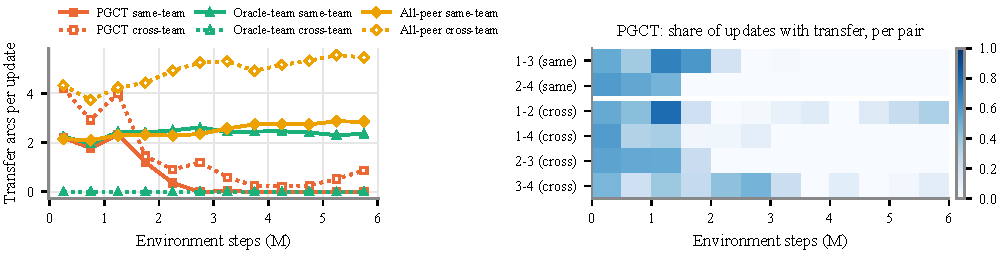
\includegraphics[width=\textwidth]{figures/fig3_critic_transfer.pdf}
\caption{Realised critic transfer on E1 (logged allocation, after warm-up; one seed\pilot). Left: directed transfer
arcs per update within (solid) and across (dotted) teams, in 0.5M-step bins. Right: for \ours{}, share of updates in
which each agent pair exchanged critic information.}
\label{fig:transfer}
\end{figure*}

\textbf{Transfer over training.} Early in training all policies are similar and the gate admits most neighbours
(transfer on 91\% of updates in the first 2M steps; Figure~\ref{fig:transfer}). As policies specialise, the gate
becomes selective: transfer happens on 37\% and 29\% of updates in 2--4M and 4--6.4M steps, compared with 82--86\% for
Oracle-team and almost 100\% for All-peer. \ours{} therefore transfers far less than either baseline while learning
faster than All-peer, suggesting that \emph{which} critics are distilled matters more than how much.

\textbf{Partners are compatible, not necessarily teammates.} In E1 the gate's later links were predominantly
across teams (agents 3--4, later 1--2; 0.03 same-team vs.\ 0.63 cross-team arcs per update after 4M steps). This is
not a failure of selection in this environment. Because observations are team-relative and the two goals are
adjacent, both teams solve the same decision problem; what differs between agents is their role (staying in the
own half vs.\ fetching shelves from the other half) and their competence. In an independent frozen-policy
evaluation, the critics of teammates were in fact \emph{less} compatible than those of non-teammates: blending a
receiver's critic with a teammate's reduced its value error less than blending it with a non-teammate's (same-team
AUROC 0.25--0.33 on four E1 checkpoints). The gate thus selects partners whose behaviour---and, empirically, whose
value predictions---are compatible, which in a team-symmetric task cuts across teams. Whether it recovers teams when
teams' objectives truly differ is the question addressed by E1-F. \todo{E1-F gate analysis}

\begin{figure}[t]
\centering
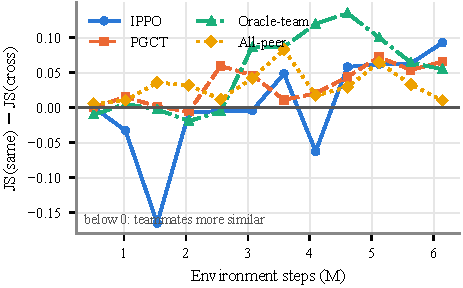
\includegraphics[width=\columnwidth]{figures/fig4_probe_js_gap.pdf}
\caption{Probe distance between teammates minus probe distance between non-teammates on E1 checkpoints (one
seed\pilot). Above zero: teammates' policies differ more than non-teammates'.}
\label{fig:jsgap}
\end{figure}

\textbf{Team information in the probe bank.} The probe distance between teammates exceeded that between
non-teammates at almost every checkpoint after 2.5M steps, for all methods (Figure~\ref{fig:jsgap}). A team-agnostic
probe bank cannot distinguish teams whose objectives look identical from the agent's team-relative viewpoint; the
v2 bank therefore includes probes in which the agent carries a shelf with no goal in view, where a team's learned
goal location determines the action. \todo{v2 gate separation on E1-F}

\section{Discussion and Limitations}
\textbf{Preliminary evidence.} All E1 numbers come from one training seed. Re-running the same seed with identical
weights reproduced IPPO exactly but not the sharing variants, which diverged after 1.4--1.6M steps (Appendix~B);
in that re-run All-peer's onset differed by two million steps. The comparison therefore requires several seeds, which
are running. \todo{report mean and 95\% interval; identify the non-deterministic operation}

\textbf{Assumptions.} \ours{} assumes a shared probe bank, local communication of model outputs, and observation
spaces in which the same probe has the same meaning for all agents. In our environment the probe bank is generated
by a fixed rule from the map layout; automatic, environment-agnostic probe construction is future work.

\textbf{Scope.} We evaluate one environment family with four agents and two teams. Larger numbers of agents and
teams, team-shared rewards, and comparisons with centralised baselines (MAPPO, SePS-style and HetDPS-style sharing)
are planned. \todo{baselines}

\section{Conclusion}
We introduced \ours{}, a decentralised method that lets each agent decide, from model outputs on a shared probe bank,
whose critic to learn from. In preliminary experiments on a two-team warehouse task, selective critic sharing
outperformed both independent learning and indiscriminate sharing and approached sharing with ground-truth
teammates, mainly by allowing agents that fell behind to learn. The gate selected compatible partners rather than
teammates in a task where both teams face the same problem; experiments with diverging team objectives and more seeds
will establish when partner selection by policy similarity coincides with team membership.

\ifdefined\ijcaistyle
  \bibliographystyle{named}
\else
  \bibliographystyle{plainnat}
\fi
\bibliography{references}

\clearpage
\appendix
\onecolumn

\section{Hyper-parameters}
\begin{table}[h]
\centering
\small
\begin{tabular}{ll}
\toprule
Setting & Value \\
\midrule
Map / agents / teams & 11$\times$10 E1 / 4 / 2 \\
Reward & individual \\
Home-zone shelf ratio & 0.5 \\
Requests per team & 2 \\
Sensor / communication range & 5 / 5 \\
Learning rate & 0.0002 \\
Entropy coef. & 0.05 \\
$\gamma$ / GAE $\lambda$ & 0.99 / 0.95 \\
Rollout / BPTT length & 1024 / 64 \\
PPO epochs / minibatches / clip & 4 / 8 / 0.2 \\
Hidden (MLP / GRU) & 128 / 128 \\
Peer-loss coef. $\lambda_{peer}$ & 0.01 \\
Gate: JS threshold / EMA $\beta$ / warm-up & 0.12 / 0.35 / 100 upd. \\
Canonical probes & 48 (fixed, zero hidden, length 1) \\
Evaluation & every 50 updates, 20$\times$500 steps, deterministic \\
\bottomrule
\end{tabular}

\caption{Settings of the from-scratch E1 comparison (identical for all methods except the donor set).}
\end{table}

\section{Reproducibility with an identical seed}
\begin{figure}[h]
\centering
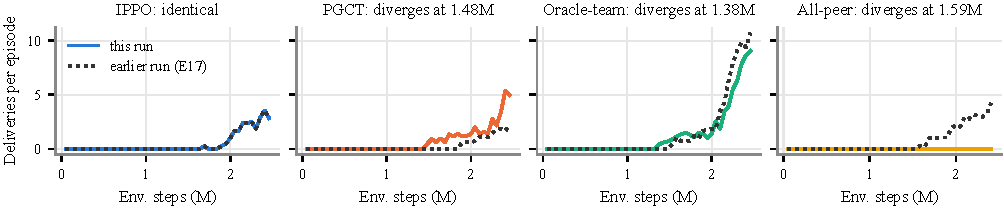
\includegraphics[width=\textwidth]{figures/figA1_reproducibility.pdf}
\caption{Two runs with the same seed and initial weights (solid: reported run; dotted: earlier interrupted run). IPPO
is reproduced exactly; the sharing variants diverge after 1.4--1.6M steps.}
\end{figure}

\section{Realised transfer per window}
\begin{table}[h]
\centering
\small
\begin{tabular}{llccc}
\toprule
Method & Window & Updates w/ transfer & Same-team arcs/upd. & Cross-team arcs/upd. \\
\midrule
PGCT & 0--2.0M & 91\% & 1.86 & 3.09 \\
 & 2--4.0M & 37\% & 0.10 & 0.73 \\
 & 4--6.4M & 29\% & 0.03 & 0.63 \\
\addlinespace
Oracle-team & 0--2.0M & 82\% & 2.26 & 0.00 \\
 & 2--4.0M & 86\% & 2.50 & 0.00 \\
 & 4--6.4M & 85\% & 2.39 & 0.00 \\
\addlinespace
All-peer & 0--2.0M & 99\% & 2.22 & 4.18 \\
 & 2--4.0M & 100\% & 2.49 & 5.10 \\
 & 4--6.4M & 100\% & 2.79 & 5.37 \\
\bottomrule
\end{tabular}

\caption{Realised transfer on E1 per training window (one seed). Arcs are directed receiver--donor links.}
\end{table}

\section{Roles in a curriculum model}
\begin{figure}[h]
\centering
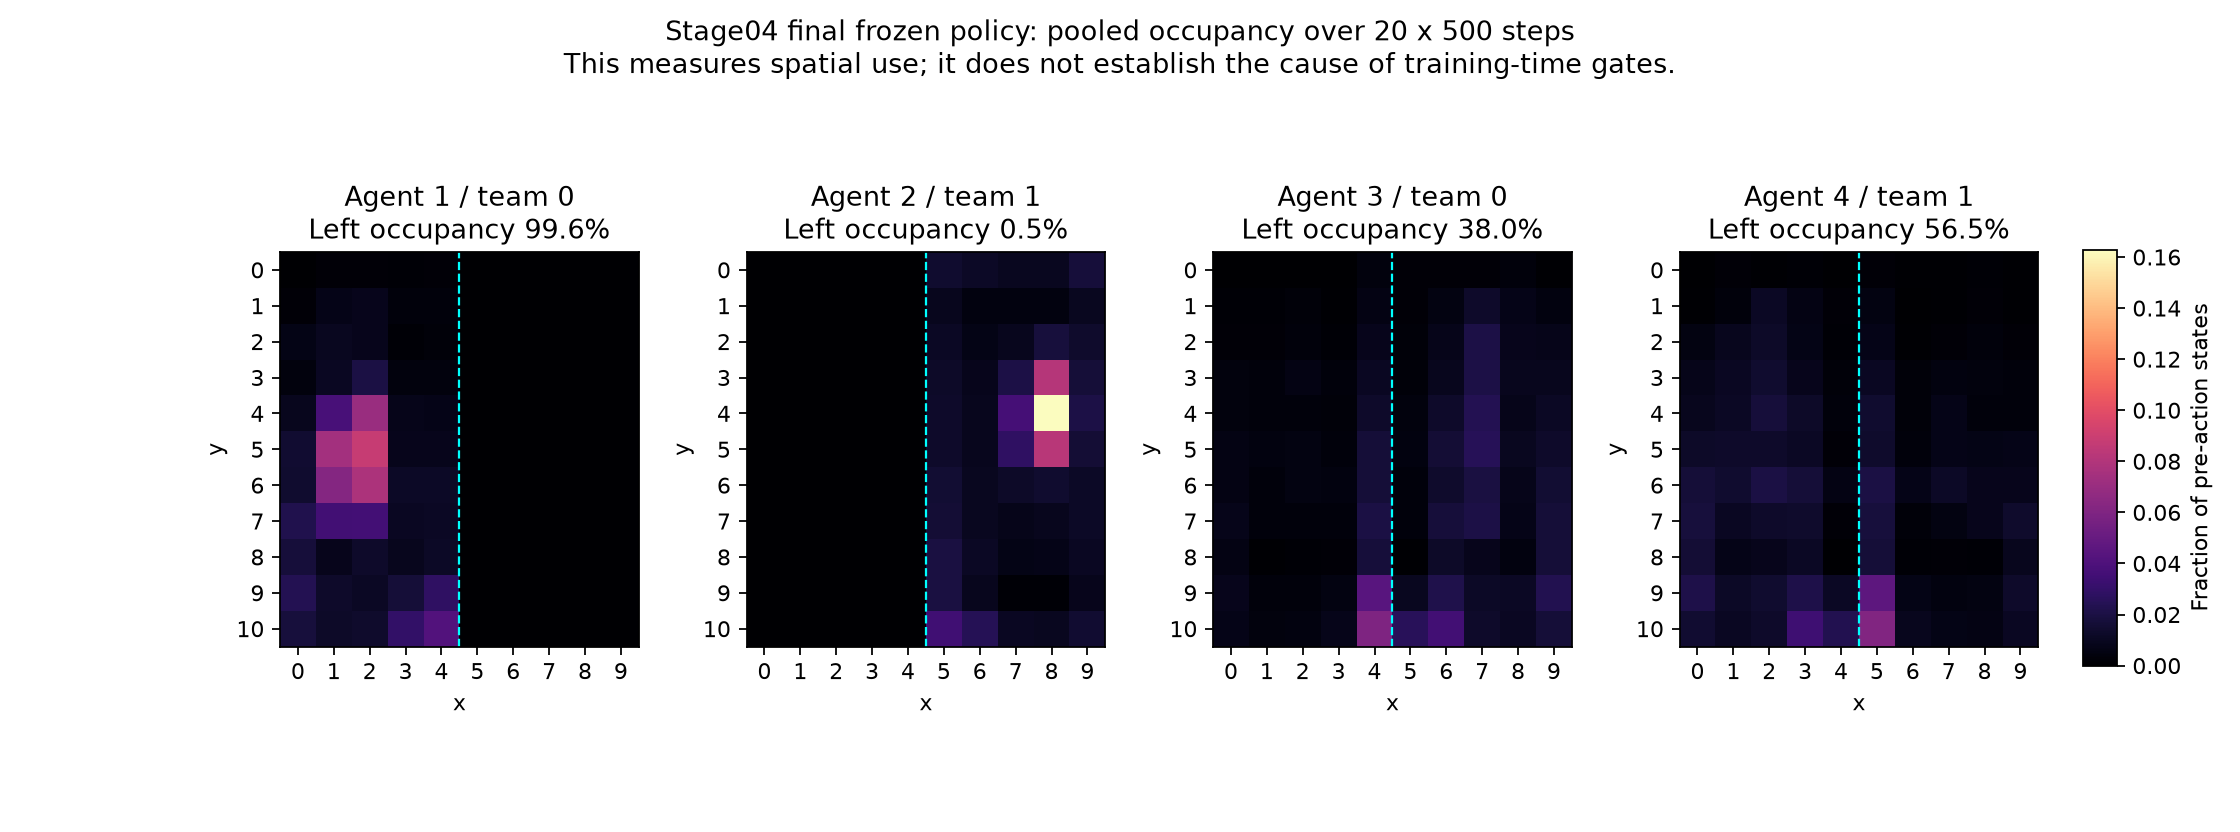
\includegraphics[width=\textwidth]{figures/stage04_occupancy.png}
\caption{Cell occupancy of a frozen curriculum model with 50\% of shelves in the other team's half (20$\times$500
steps). Agents 1 and 2 stay in their team's half; agents 3 and 4 fetch shelves from the other half and are the pair
the gate linked most often.}
\end{figure}

\end{document}
